\documentclass[a4paper,12pt]{article}

% Paquetes básicos
\usepackage[utf8]{inputenc}
\usepackage[T1]{fontenc}
\usepackage[spanish]{babel}
\usepackage{graphicx}
\usepackage{xcolor}
\usepackage{lipsum}
\usepackage{geometry}
\geometry{top=3cm, bottom=3cm, left=2.5cm, right=2.5cm}

% Paquetes para diseño
\usepackage{titlesec}
\usepackage{fancyhdr}
\usepackage{amsmath}
\usepackage{amssymb}
\usepackage{hyperref}

% Paquetes para el entorno lstlisting
\usepackage{listings}
\usepackage{inconsolata}

% Paquete para fondo
\usepackage{background}

% Configuración de lstlisting
\lstset{
    language=Python,
    basicstyle=\ttfamily\small,
    keywordstyle=\color{blue}\bfseries,
    stringstyle=\color{teal},
    commentstyle=\color{gray}\itshape,
    numbers=left,
    numberstyle=\tiny\color{gray},
    backgroundcolor=\color{black!5},
    frame=single,
    rulecolor=\color{black!50},
    breaklines=true,
    captionpos=b,
    showstringspaces=false
}

% Configuración de título
\titleformat{\section}{\normalfont\Large\bfseries}{\thesection}{1em}{}

% Información del documento
\title{
    \vspace{-2cm}
    
\includegraphics[width=0.3\textwidth]{images/fccee.jpg} \\ % Cambia el logo si es necesario
    \LARGE Ingeniería Informática + ADE\\
    \large Universidad de Granada (UGR)\\[1cm]
}
\author{\textbf{Autor:} Ismael Sallami Moreno}
\date{\textbf{Asignatura:} Resúmenes de Contabilidad Financiera I Tema 5: Inmovilizaciones materiales
}
\usepackage{mathpazo}
\pagestyle{fancy}
\fancyhf{}
\fancyhead[L]{\textbf{\textsf{\leftmark}}}
\fancyhead[R]{\textbf{\textsf{\thepage}}}
\fancyfoot[C]{\thepage}

% Configuración del fondo
\backgroundsetup{
    scale=1,
    color=black,
    opacity=0.2,
    angle=0,
    position=current page.south,
    vshift=0pt,
    hshift=0pt,
    contents={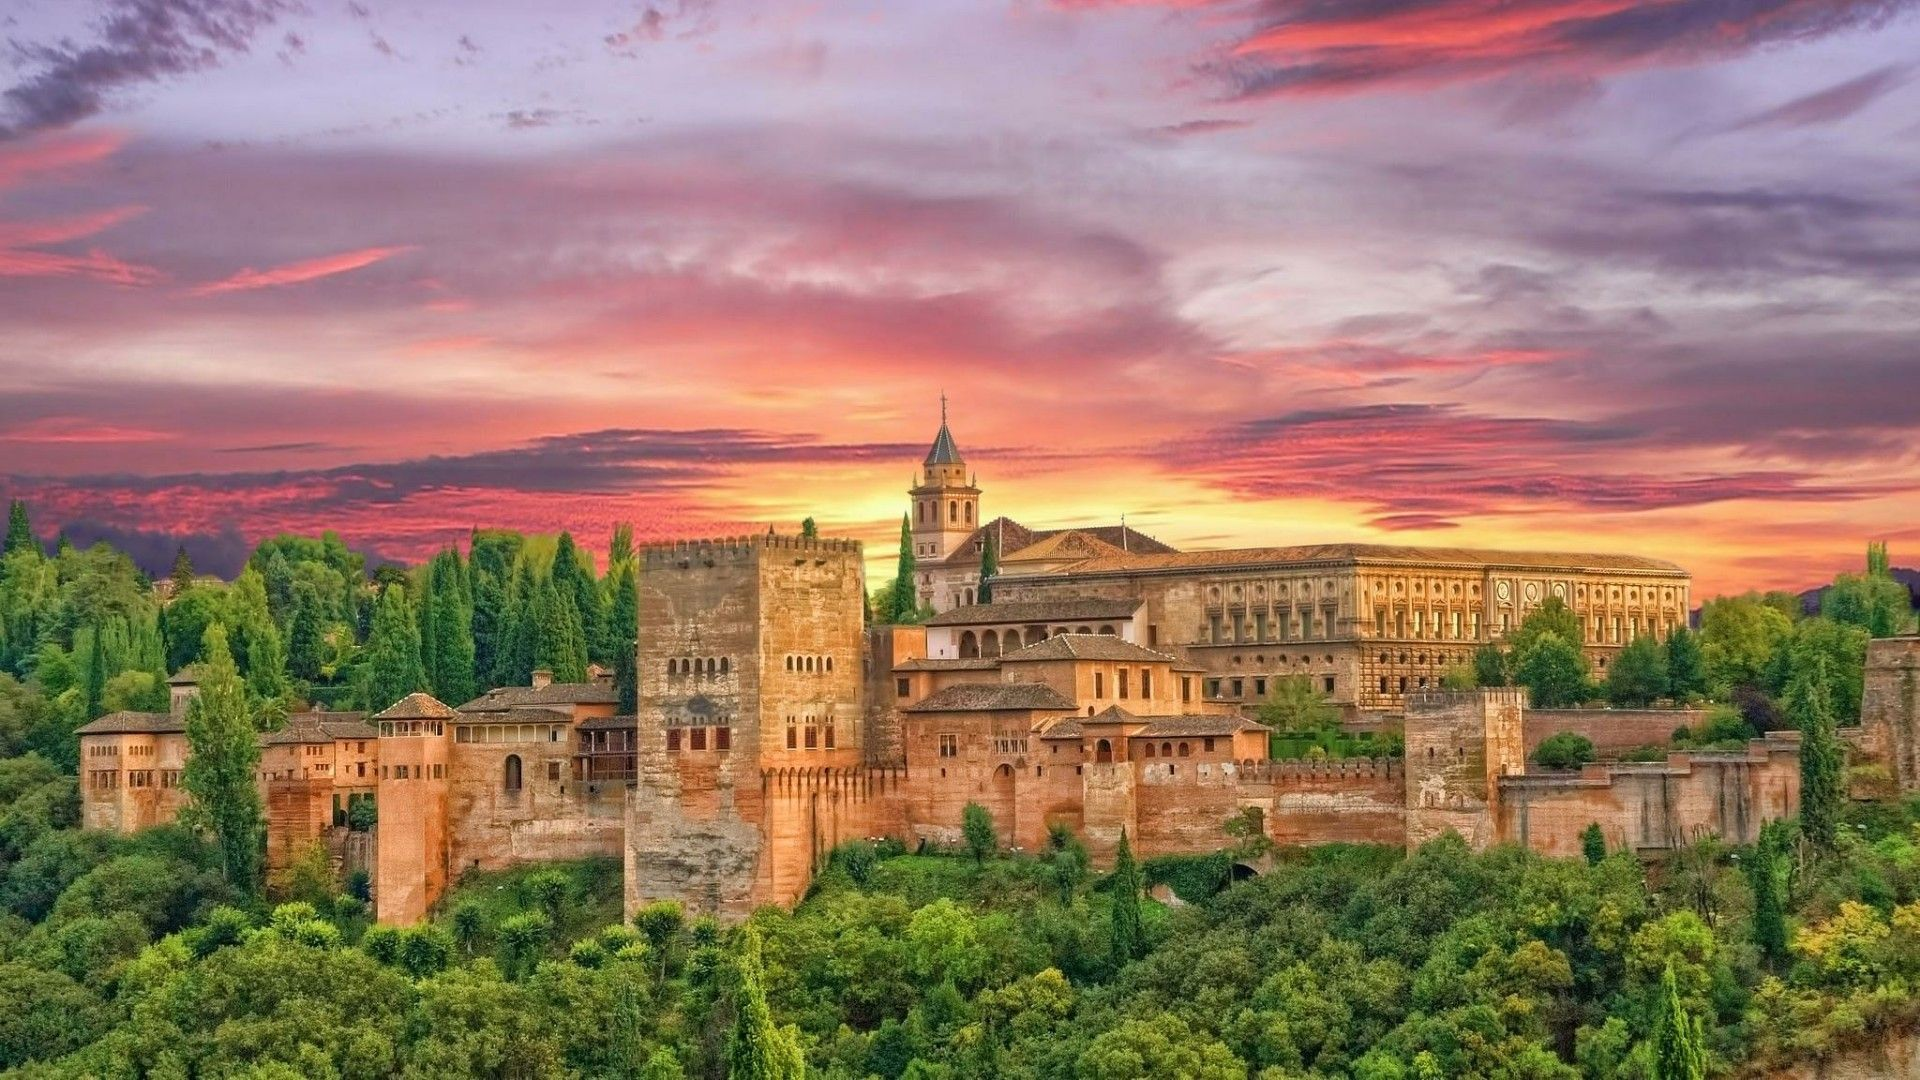
\includegraphics[width=\paperwidth,height=\paperheight,keepaspectratio]{images/granada.jpg}}
}

% Inicio del documento
\begin{document}

% Portada
\maketitle
\thispagestyle{empty}

\begin{center}
    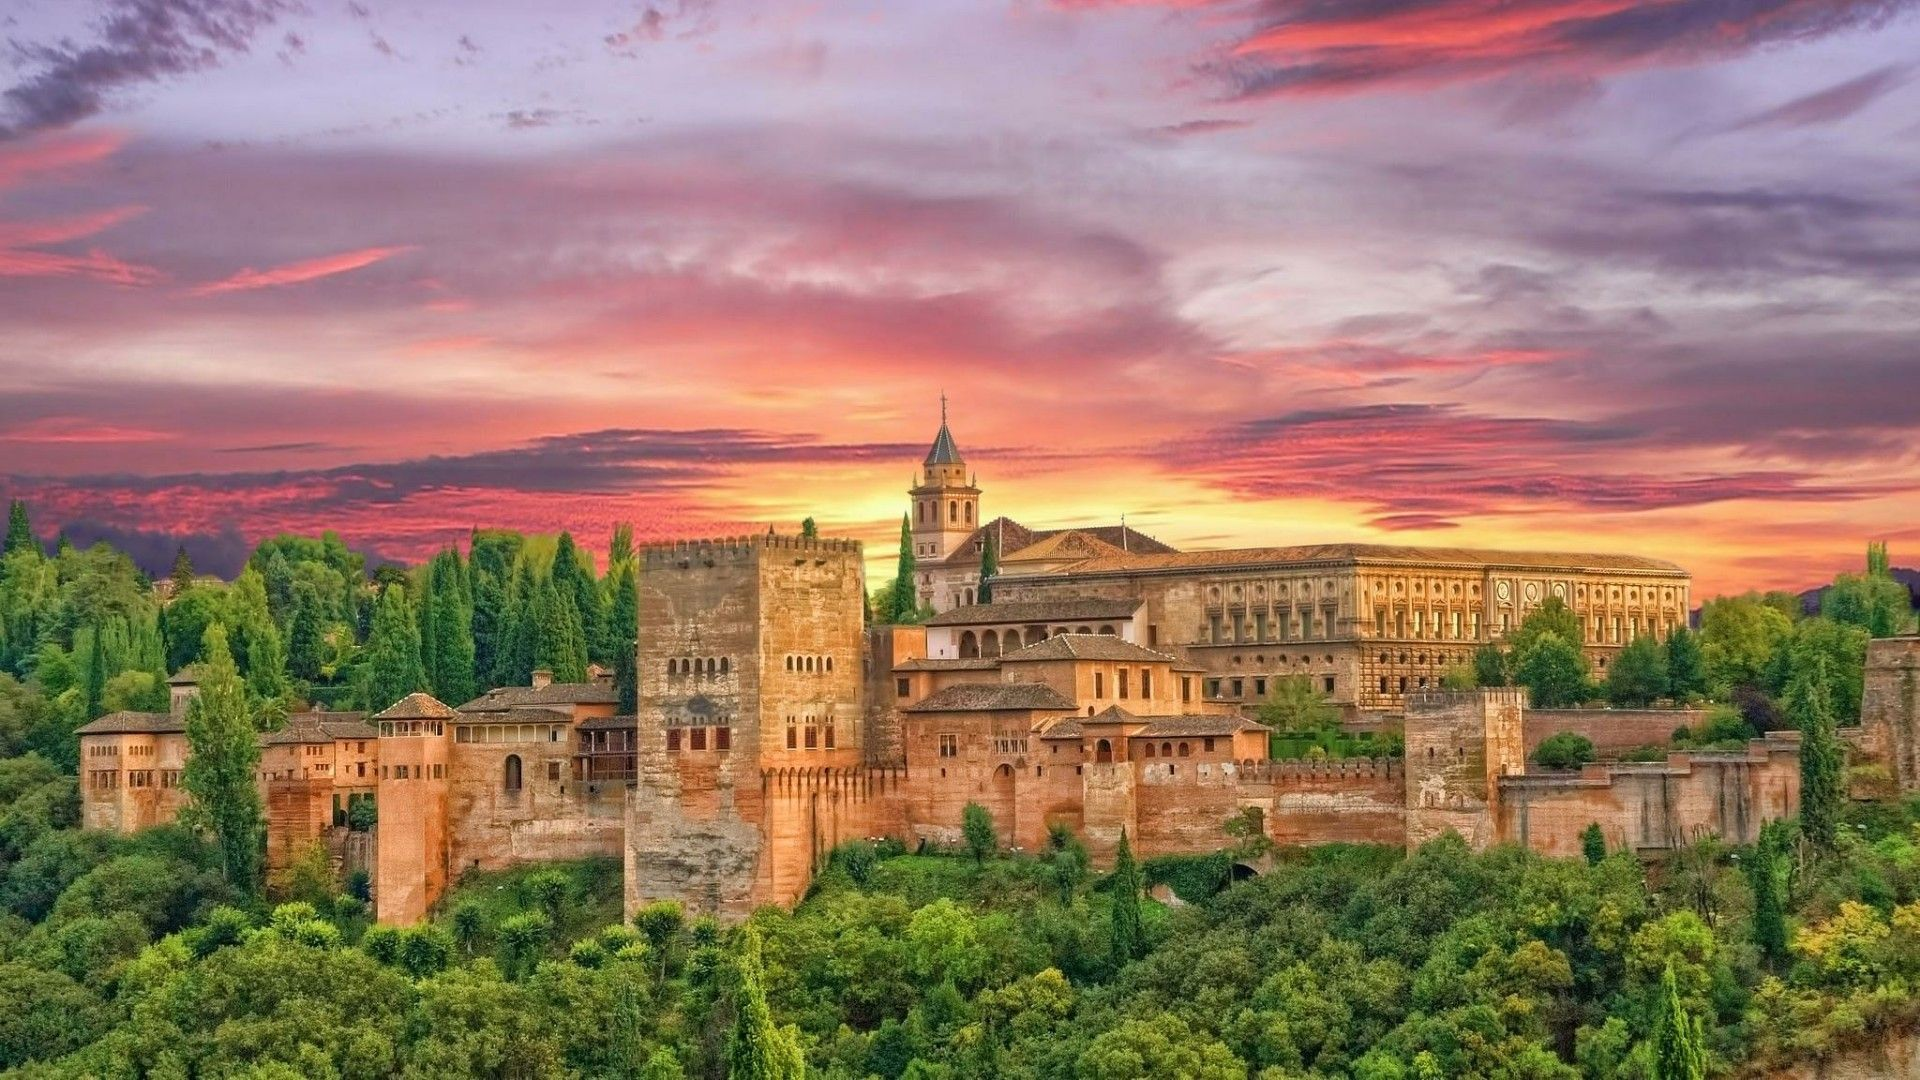
\includegraphics[width=\textwidth,height=0.4\textheight,keepaspectratio]{images/granada.jpg} \\ % Añade tu imagen de fondo
    \vfill
\end{center}

\newpage

% Índice (opcional)
\tableofcontents
\newpage

\section{Concepto, características y clasificación del inmovilizado}

\subsection{Concepto de inmovilizado}
Bienes, derechos y otros recursos controlados económicamente por la empresa, resultantes de sucesos pasados, de los que se espera que la empresa obtenga beneficios o rendimientos económicos en el futuro.

\subsection{Definición de activo no corriente}
Comprende los activos destinados a servir de forma duradera en las actividades de la empresa, incluidas las inversiones financieras cuyo plazo de vencimiento sea superior a un año.

\subsubsection{Características del activo no corriente}
\begin{itemize}
    \item largo plazo
    \item no están destinados a ser vendidos
    \item incluye las inversiones financieras a largo plazo
    \item se deprecia de manera irreversible y sistemática (amortización técnica) y también se puede depreciar de modo reversible (deterioros de valor)
\end{itemize}

\subsection{Definición de activo corriente}
Comprende los activos vinculados al ciclo normal de explotación que la empresa espera a vender, consumir o realizar. El ciclo de explotación no excederá un año.

\subsection{Ciclo normal de explotación}
Periodo que transcurre entre dos momentos de tiempo: 
\begin{enumerate}
    \item momento de adquisición de bienes que se invierten (proceso productivo)
    \item realización de los bienes de manera efectiva(recuperación de la inversión)
\end{enumerate}

\subsection{Clases de inmovilizado}

En función del subgrupo:
\begin{itemize}
    \item 20: Inmovilizado intangibles
    \item 21: Inmovilizado materiales
    \item 22: Inmovilizado inmobiliarias
    \item 23: Inversiones materiales en curso
    \item 24: Inversiones financieras en partes vinculadas
    \item 25: Inversiones financieras a largo plazo
    \item 26: Fianzas y depósitos constituidos a largo plazo
    \item 27: Amortización acumulada del inmovilizado
    \item 28: Deterioro de valor del Inmovilizado
\end{itemize}

\end{document}

\section{Concepto y características del inmovilizado material}